\section{Ejercicio 1}

\subsection{Introducción}

En este ejercicio se plantea una máquina de estados para controlar la carga de un tanque de agua mediante la utilización de dos bombas independientes. \par
La cátedra solicita una implementación mediante una máquina de Moore, la cual se caracteriza porque las salidas no dependan de las entradas. Estas últimas servirán para realizar cambios de estado y controlar el flujo general de la máquina. Por otro lado, cada estado tendrá asociado una salida. La implementación característica de una máquina de Moore se presenta a continuación:

\begin{figure}[H]
\begin{center}
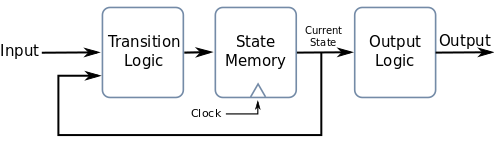
\includegraphics[scale=0.8]{Ejercicio1/Imagenes/moore}
\caption{Máquina de Moore}
\end{center}
\label{Maquina_de_Moore}
\end{figure}

Los sensores $S$ e $I$ ubicados en la parte superior e inferior del tanque respectivamente, actuarán como las entradas de la máquina de estado, su valor será $1$ al detectar agua y $0$ en caso contrario. Para la implementación se utilizarán cuatro estados los cuales indicarán el estado de funcionamiento de las bombas como se muestra en la tabla (\ref{Estados}). \par
Para representar dichos estados son necesarios dos bits, como dichos bits representarán el estado de las bombas, los estados coincidirán con las salidas de la máquina de Moore.
 

\begin{table}[H]
	\begin{center}
	\scalebox{0.9}{
		\begin{tabular}{c|c|c}
		Estado & $Q_1$                  & $Q_0$ \\ \hline
		A      & \multicolumn{1}{c|}{0} & 0     \\
		B      & \multicolumn{1}{c|}{0} & 1     \\
		C      & \multicolumn{1}{c|}{1} & 0     \\
		D      & \multicolumn{1}{c|}{1} & 1    
		\end{tabular}
	}
	\caption{Estados utilizados}
	\end{center}
	\label{Estados}
\end{table}



 Donde dichos estados representan:\newline
 A: Ninguna bomba está encendida \newline
 B: La bomba 0 está encendida \newline
 C: La bomba 0 está encendida \newline
 D: Ambas bombas están encendidas \newline
 \par
 
 A continuación, se representa el diagrama de estados y la tabla de transciones de nuestra máquina.
 
 \begin{figure}[H]
\begin{center}
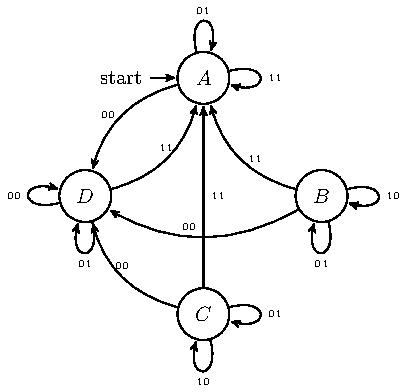
\includegraphics[scale=0.9]{Ejercicio1/Diagramas/Transiciones}
\caption{Diagrama de estados}
\end{center}
\label{Diagrama_de_estados}
\end{figure}




\begin{table}[H]
\begin{center}
\scalebox{0.7}{
\begin{tabular}{c|cc|cc}
\multirow{2}{*}{\begin{tabular}[c]{@{}c@{}}Estado \\ Actual\end{tabular}} & \multicolumn{2}{c|}{S=0}     & \multicolumn{2}{c}{S=1}     \\
                                                                          & I=0                    & I=1 & I=0                    & I=1 \\ \hline
A                                                                         & \multicolumn{1}{c|}{D} & A   & \multicolumn{1}{c|}{X} & A   \\
B                                                                         & \multicolumn{1}{c|}{D} & B   & \multicolumn{1}{c|}{B} & A   \\
C                                                                         & \multicolumn{1}{c|}{D} & C   & \multicolumn{1}{c|}{C} & A   \\
D                                                                         & \multicolumn{1}{c|}{D} & D   & \multicolumn{1}{c|}{X} & A	\\
\end{tabular}
}
\label{Tabla_de_transiciones_Ej1}
\caption{Tabla de transiciones}
\end{center}
\end{table}



Desarrollando las tablas obtenmos los siguientes Karnaugh:
%Mapas de Karnaugh 
\subsection{Implementación}



\begin{center}
	\hspace*{\fill}
   \begin{tikzpicture}[x=1cm,y=1cm]
    \K[x bits = 2, y bits = 2, label={$Y_1$},
       variable names = {$I$,$S$,$Q_1$,$Q_0$,}]
    { 
      0000,1,    
      0001,1,   
      0010,1,   
      0011,1,       
      0100,0, 
      0101,0,
      0110,1,
 	  0111,1,
 	  1000,X,    
      1001,0,   
      1010,1,   
      1011,X,       
      1100,0, 
      1101,0,
      1110,0,
 	  1111,0,
    }
    \newcommand*{\myKG}[4][0.1]{\KG[x bits = 2,y bits = 2,group opacity = #1,
                  #2]{#3}{#4}}
    \myKG     {group color = red,  group distance=0.35}{0010}{0000}
    \myKG     {group color = pink,  group distance=0.35}{0010}{0111}
    \myKG     {group color = purple,  group distance=0.35}{1010}{0011}


    %=====================================================================
    % in picture comments
    %=====================================================================

    \path (1,-3.5) node[anchor = north, align = left] (eq1){%
    $D_1 = 
       \ul{red}{$\ol{I}\,\ol{S}\,$}
       +\ul{pink}{${Q_1}\,\ol{I}\,$}  
       +\ul{purple}{${Q_1}\,\ol{S}\,$}  
    $};
    
  \end{tikzpicture}
	\hspace{2mm}
   \begin{tikzpicture}[x=1cm,y=1cm]
    \K[x bits = 2, y bits = 2, label={$Y_1$},
       variable names = {$I$,$S$,$Q_1$,$Q_0$,}]
    { 
      0000,1,    
      0001,1,   
      0010,1,   
      0011,1,       
      0100,0, 
      0101,1,
      0110,0,
 	  0111,1,
 	  1000,X,    
      1001,1,   
      1010,0,   
      1011,X,       
      1100,0, 
      1101,0,
      1110,0,
 	  1111,0,
    }
    \newcommand*{\myKG}[4][0.1]{\KG[x bits = 2,y bits = 2,group opacity = #1,
                  #2]{#3}{#4}}
    \myKG     {group color = red,  group distance=0.35}{0010}{0000}
    \myKG     {group color = pink,  group distance=0.35}{0011}{0101}
    \myKG     {group color = purple,  group distance=0.35}{1011}{0001}


    %=====================================================================
    % in picture comments
    %=====================================================================

    \path (1,-3.5) node[anchor = north, align = left] (eq1){%
    $D_1 = 
       \ul{red}{$\ol{I}\,\ol{S}\,$}
       +\ul{pink}{${Q_1}\,\ol{I}\,$}  
       +\ul{purple}{${Q_1}\,\ol{S}\,$}  
    $};
    
  \end{tikzpicture}
	\hspace{2mm}
	\hspace*{\fill}
\end{center}

Dando como resultado los siguientes circuitos:

\begin{figure}[H]
\begin{center}
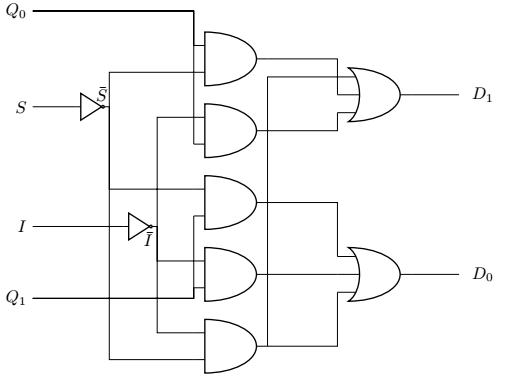
\includegraphics[,scale=0.5]{Ejercicio1/Circuitos/Logica1}
\caption{Transiciones Caso I}
\end{center}
\label{Transiciones_Caso_I}
\end{figure}

 \begin{figure}[H]
\begin{center}
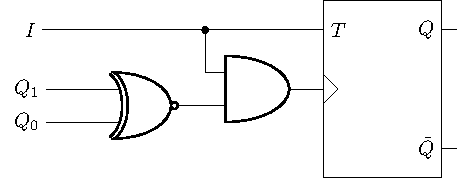
\includegraphics[scale=1]{Ejercicio1/Circuitos/Logica2}
\caption{Transiciones Caso II}
\end{center}
\label{Transiciones_Caso_I}
\end{figure}

 \begin{figure}[H]
\begin{center}
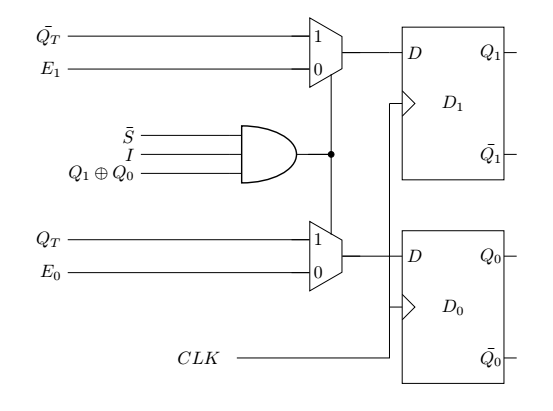
\includegraphics[,scale=0.5]{Ejercicio1/Circuitos/Sumalogica}
\caption{Diagrama de estados}
\end{center}
\label{Diagrama_de_estados}
\end{figure}

